% !TeX root = main.tex
\documentclass[french]{beamer}

\usepackage{defPreamble}

\begin{document}

\pdfcompresslevel=0
\pdfobjcompresslevel=0

\frame{\titlepage}
\begin{frame}{Table of Contents}

\tableofcontents
\end{frame}


%
% ------- REAL START -------------
%

\section{Rappel: But du TP}
\bframe{
    \begin{itemize}
      \item Implémenter un serveur établissant une connection avec plusieurs connections connections clients
      afin de jouer au \quo{guessing game} avec chacun simultanément
    \end{itemize}
    \vspace{0.3cm}
    
    Les principaux défis de ce TP sont:
    \begin{itemize}
        \item L'implémentation de l'architecture client/serveur TCP correspondante
        \item Manipuler les appels liés aux sockets (création, écoute, attente, connection\ldots)
        \item Gérer simultanément un proccessus enfant par client plus un parent qui attend une connection d'un client puis crée un enfant pour jouer avec lui.
    \end{itemize}
}

\section{TADs \& leurs relations}
\subsection{Décomposition modulaire}

\bframes{
    4 modules (+ \texttt{main.c}) ont été créés pour la réalisation du TP\@:
    \begin{enumerate}
        \item \code{main.c}: contient le code principal du programme \& appelle les fonctions appropriées
              des autres modules.\\

        \item \code{copy.c}: contient 4 fonctions, sert à gérer la copie des fichiers et répertoires,
              de définir quand est-ce qu'un fichier est considéré comme \quo{modifié}\ldots \\

        \item \code{files.c}: contient 11 fonctions, servant à gérer les fichiers et leurs attributs.\\
        \item \code{optprsr.c}: contient 3 fonctions, servant à gérer les options passées en paramètres. (repris du tp d'avant)\\

        \item \code{util.c}: contient 9 fonctions, servant divers usages allant de la gestion d'erreurs à la gestion de chaînes de caractères, en passant par des wrappers qui incluent lesdites fonctions de gestions d'erreurs.\\
    \end{enumerate}
}
%

\subsection{Structures de données utilisées}
\bframes{
    L'implémentation de structure n'a pas été nécessaire.
}

\subsection{Décomposition fonctionnelle}
\bframes{
    \begin{enumerate}
        \item[(1)]  \code{main.c}\\
              \begin{itemize}
                  \item \code{handleArgs}: Permet de gérer la totalité des arguments passés (les fichiers/dossiers (obligatoire) et les arguments optionnels tels que \code{-a} et \code{-f})
                        appelle \code{optprsr.c} pour parse/extraire les arguments obligatoire \& optionnels et leurs fait
                        correspondre le bon chant du bitfield \code{ST\_\ldots}.

                        \vspace{0.3cm}

                  \item \code{main}: Gère les differentes possibilités de copier les fichiers/dossiers (seulement 2 fichiers, 1 fichier et un dossier, 1 (ou plus) dossier(s) vers 1 dossier et les arguments optionnels)
                        i.e. appelle \code{handleArgs} récupérer le \textit{state} (bitfield \code{ST\_\ldots}) pour ensuite déléguer aux fonctions du module \code{copy} en fonctions des différents
              \end{itemize}\end{enumerate}
}
\bframes{
    \begin{enumerate}
        \item[(2)] \code{copy.c}
        \begin{itemize}
            \item \code{is\_modified}: Compare les temps de la dernière modification, et leurs tailles. S'il y a une différence entre les deux, le fichier sera remplacé par le nouveau
            \item \code{copy}: Copie le contenu d'un fichier à un autre (code de l'exemple du chapitre 7: I/0 du cours, avec quelques modifications)
            \item \code{copy\_ifneeded}: Vérifie si deux fichiers diffèrent et copie si c'est le cas
            \item \code{ultra-cp-single}: Si le fichier passé en argument a été modifié\\ $\Rightarrow$ copie à la destination passée en argument;
            en changeant les permissions du fichier copié si demandé en option.
            \item \code{ultra\_cp}: Backup le dossier passé en argument à la destination passée en argument. Traverse récursivement tous les 
            dossiers en créant les dossiers nécessaires au passage et appelles \code{ultra-cp-single} pour chaque fichier rencontré.
        \end{itemize}
    \end{enumerate}

}

\bframes{
    \begin{enumerate}
        \item[(3)] \code{files.c}
            \begin{itemize}
                \item Les fonctions \code{is\ldots}: Vérifient si l'argument est quelque chose. Ex: isDir vérifie si l'argument est un directory
                \item \code{computePerm}: Retrouve les permissions d'un fichier donné
                \item \code{exists}: Dit si un fichier donné existe. Retourne un erreur sinon
                \item \code{concat\_path}: Concatène le path d'un fichier et de son directory parent
                \item \code{absPath}: Retourne le path absolu d'un fichier
                \item \code{getFileName}: Retourne le vrai nom d'un fichier à partir du path absolu
                \item \code{listEntry}: Print les informations d'un fichier: type, permissions, taille, heure de modification et son path
                \item \code{listEntryNoIn}: Idem, mais sans inode en argument
                \item \code{list\_dir}: Print les informations de chaque fichier dans un directory
            \end{itemize}
    \end{enumerate}

}

\bframes{
    \begin{enumerate} 
        \item[(4)] \code{optprsr.c}
            \begin{itemize}
                \item \code{checkEnoughArgs}: Vérifie que suffisamment d'arguments obligatoires ont été entrées
                \item \code{parseArgs}: Parse les arguments obligatoires. Ici, ce sont les fichiers et dossiers sources et la destination
                \item \code{parseOptArgs}: Parse les arguments optionnels. Ici, ce sont \code{-a} et \code{-f}
            \end{itemize}
    \end{enumerate}
}
\bframes{
    \begin{enumerate} 
        \item[(5)] \code{util.c}
            \begin{itemize}
                \item \code{tryalc}: Vérifie que malloc a été effecté sans problème
                \item Les fonctions \code{hdl...}: Gèrent multiples erreurs avec les fichers (ouvrir, fermer etc.)
                \item \code{stat\_s} et \code{lstat\_s}: Permettent d'obtenir les informations d'un fichier (comme stat et lstat dans bash)
            \end{itemize}
    \end{enumerate}
    %  \end{enumerate}

}

%
%


\section{Tests realisés pour valider le fonctionnement du TP}
\bframe{
Les tests réalisés ont étés les suivants:

%\item \code{./digest -f file1 file2 ...[-t <hashMethod>]} \\
{\scriptsize \code{./ultra-cp dossier\_1 [[$\cdots$ dossier\_n] [fichier\_1 $\cdots$
    fichier\_n]]}\\

    $\qquad \qquad \qquad \qquad \qquad$ \code{[destination] [-a] [-f] }}

Selon les utilisations suivantes: (commentaire copié du code)
\begin{enumerate}
    \item[1.] Just 1 file/folder $\Rightarrow$ print/ls contents
    \item[2.] If only 2 files are given $\Rightarrow$ create/replace the file
    \item[3.] If multiple files \& folder and \quo{dest} exists $\Rightarrow$ create/replace architecture in \quo{dest}
    \item[4.] If -a is passed, change the permissions
    \item[5.] If -f is passed, links are copied as links (stored in optional state)
\end{enumerate}

}

\bframe{
    \vspace{-0.2cm}
    {\scriptsize Soit le dossier \code{res/} contenant les fichiers suivants:}
    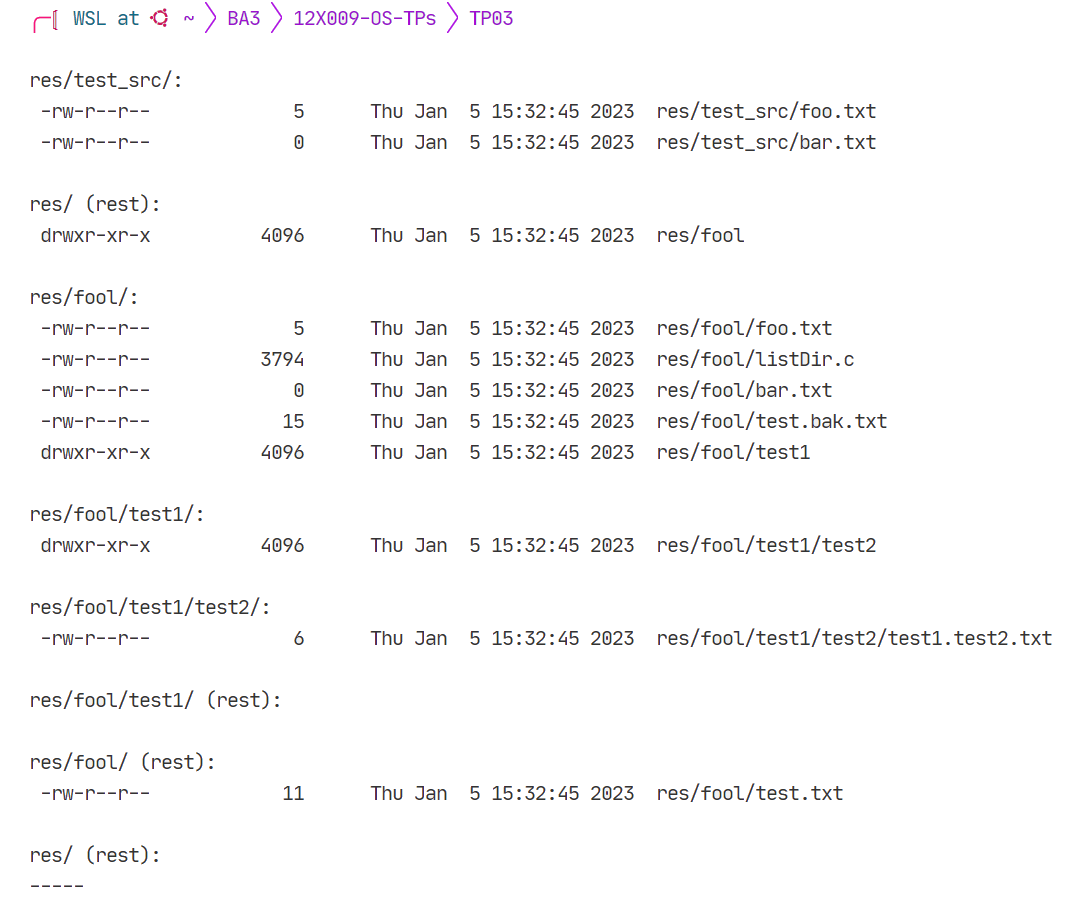
\includegraphics[scale=0.48]{images/os-tp3-prez-resDir2.png}
}

\bframe{
    Les tests suivants ont été réalisés:
  
  \begin{enumerate}
      \item \code{./ultra-cp res/fool tmp}
      \item \code{./ultra-cp res/fool/bar.txt tmp}
      \item \code{./ultra-cp  res/test\_src/foo.txt}
      \item \code{./ultra-cp  res/test\_src/foo.txt foo}
      \item \code{./ultra-cp res/test\_src/bar.txt res/test\_src/foo.txt  res/test\_src res/fool}
   
  \end{enumerate}
}


\bframe{
    Les tests suivants ont été réalisés:
  
  \begin{enumerate}
      \item \code{./ultra-cp res/fool tmp -f}
      \item \code{./ultra-cp res/fool/bar.txt tmp.txt}
      \item \code{./ultra-cp  res/test\_src/foo.txt}
      \item \code{./ultra-cp  res/test\_src/foo.txt foo}
      \item \code{./ultra-cp res/test\_src/bar.txt res/test\_src/foo.txt} \\
      $\qquad \qquad \quad$ \code{res/test\_src res/fool -f}
  \end{enumerate}
  La dernière commande donnant l'output suivant:
}

\bframe{
    \vspace{-0.2cm}
    \includegraphics[scale=0.48]{images/os-tp3-prez-lastTest.png}
}




%
\section{Réponses aux questions (de l'énoncé du TP)}
\begin{frame}{\secname}
%

\begin{itemize}
    \item 
    \vspace{0.3cm}

    \begin{itemize}
        \item  
    \end{itemize}
   
\end{itemize}

\end{frame}


\section{Réponses aux questions (générales)}

\begin{frame}{\secname}
\end{frame}

%
%
\end{document}
